\chapter{Algoritmo ottimizzato tramite decomposizioni bilanciate}
\label{cap:3}
In questo capitolo viene presentata un'ottimizzazione al problema descritto nel capitolo precedente.
Tale ottimizzazione si basa sul principio delle decomposizioni bilanciate.
Si fa vedere, inoltre, come vengono modificati i precedenti dettagli implementativi.

\section{Decomposizioni Bilanciate di un albero}
\label{cap:3 par:1}
Nel precedente capitolo, dato un albero ben colorato $ T $ vengono considerate tutte le possibili decomposizioni dell'albero, comprese quelle per cui $ T $ pu\`o essere scomposto in due alberi $ T' $ e $ T'' $ con cardinalit\`a molto diverse (e.g. $ |T'|=k-1 $ e $ |T''| = 1 $).\\ 
Si vuole andare a dimostrare, invece, in questa sezione che dato un albero T \`e sempre possibile ricavare una decomposizione bilanciata dell'albero scomponendolo, perci\`o,  in due alberi $ T' $ e $ T'' $ le cui cardinalit\`a risultino ``bilanciate''.
\\
Prima di poter enunciare e dimostrare il risultato principale occorre dare delle nozioni preliminari.

\newtheorem{definizione}{Definizione}[section]

\begin{definizione}
	\label{definizioneDeco} 
Sia $T_r$ un albero, con k nodi, radicato nel nodo r.
Diremo che la coppia (A,B), dove  A e B sono due alberi ottenuti a partire dai nodi di $T_r$, \`e una decomposizione per l'albero $ T_r $ se:
\begin{itemize}
	\item $| A | + | B | = k$
	\item $A \cap B = \{r\}$.
\end{itemize}
\end{definizione}


\begin{definizione}
\label{lemmaDeco}
Dato un albero $ T $ con $ k $ nodi, diremo che $ (A,B) $ \`e una decomposizione $ f(k) $-bilanciata se:
\begin{equation*}
	\max{ \{|A| , |B| \} }  \le  f(k)
\end{equation*}
\end{definizione}





\begin{definizione}
Per ogni nodo $ v $ di un albero $ T $, le diramazioni di $ T $  rispetto a $ v $, sono tutti i sottoalberi massimali di $ T $ non contenenti $ v $. 
Per ogni $ v \in T $, si definisce $\alpha(v)$ come il massimo numero di nodi tra le diramazioni di $ v $.\\
Un nodo $ v $ di un albero $ T $ con $ n $ nodi, \`e un nodo centroide se $\alpha(v)\le\frac{n}{2}$.
\end{definizione}\mbox{}

Il centroide di un albero non \`e necessariamente unico, infatti Jordan \cite{jordan1869assemblages}  ha dimostrato che, dato un albero $ T $ con $ n $ nodi:
\begin{enumerate}
	\renewcommand{\labelenumi}{\roman{enumi}}
	\item $ T $ ha un singolo centroide $ v $ e $\alpha(v) < \frac{n}{2}$, oppure
	\item$ T $ ha due nodi centroidi (adiacenti) $v_1$ e $v_2$ tali che $\alpha(v_1) = \alpha(v_2) = \frac{n}{2}$, in questo caso il numero di nodi $ n $ \`e pari.
\end{enumerate}

Esistono diversi algoritmi per la ricerca del centroide, quello utilizzato in questa tesi \`e un algoritmo con complessit\`a temporale lineare nel numero di nodi. \\
Il primo passo da effettuare \`e determinare in un albero $ T $, con $ n $ nodi, $\alpha(v)$ per ogni nodo $ v \in T$.\\
Innanzitutto per ogni nodo $ v\in T $ indichiamo con $ \eta(v) $ il numero di nodi presenti nel sottoalbero radicato in $ v $ di $ T $.\\
A questo punto si procede ad una visita $ DFS $ sull'albero, memorizzando $ \forall v\in T $ il rispettivo valore $ \eta(v) $, che sar\`a calcolato nel seguente modo 
\[\eta(v) = 1 + \sum_{\substack{u \ figlio \ di \ v \ in \ T} } { \eta(u)}\].
Una volta conclusa la visita, si pu\`o determinare $ \alpha(v) $ per ogni nodo $ v $ in $ T $, come segue
\[ \alpha(v) = \max\{ \max_{\substack{u \ figlio \ di \ v \ in \ T}} {\eta(u)} \ , \ n - \eta(v) \} \]
\\
Una volta calcolato il valore di $ \alpha(v) $ per ogni $  v \in T $ si verifica per quali valori  risulta $\alpha(v)\le\frac{n}{2}$.\\
Nel caso ci fosse un unico nodo $ v $ che soddisfa la precedente espressione, come in (i),  allora tale nodo rappresenta l'unico  centroide dell'albero $ T $.
Nel caso, invece, ce ne fossero due, come definito in (ii), per esempio $ v_1 $ e $ v_2 $,  l'albero $ T $ conterr\`a due centroidi, rispettivamente $ v_1 $ e $ v_2 $.\\
Per verificare che l'algoritmo ha una complessit\`a $ T(n) $ lineare sul numero di nodi.
Basta notare che la visita $ DFS $ su un albero $ T $ di $ n $ nodi richiede un tempo $ O(n) $ per essere completata.
A questa quantit\`a va sommato il tempo necessario per determinare per ogni nodo $ v $ di $ T $ il rispettivo grado, che indichiamo con $ \delta(v) $, anche questo richiede un tempo lineare sul numero di nodi $ n $.
In particolare mettendo insieme quanto detto finora quello che si ottiene \`e
\[  T(n) = O(n + \sum_{v}(1+\delta(v)))= O(n + n + \sum_{v}\delta(v)) = O(n+n+n)=O(n)\] 
Nell'esempio \ref{es1} si pu\`o vedere l'applicazione dell'algoritmo per la ricerca del centroide.
	\begin{figure}[htbp]
		\centering
		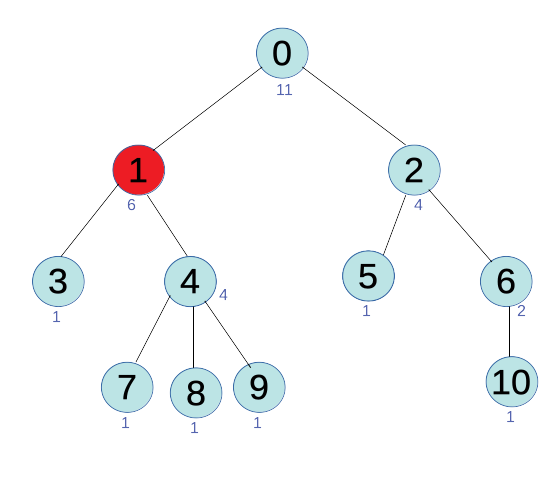
\includegraphics[width=5cm]{capitolo3/grafo2}
		\caption{Albero $ T $  per la ricerca del centroide} 
		\label{fig:2}
\end{figure}
\mbox{}\\

\newtheorem{esempio}[definizione]{Esempio}
\begin{esempio}
	\label{es1}
Si consideri l'albero T in figura \ref{fig:2} per la ricerca del nodo centroide.
Per ogni nodo $ v $ di $ T $ numerato da 0 a 10,  viene calcolato $\alpha(v)$ . \\
Quello che si ottiene \`e :


\begin{center}
	\begin{tabular}{ c c c c c  }
		$\alpha(0) = 6$ & & $\alpha(1) = 7$ & & $\alpha(2) = 5$ \\ 
		$\alpha(3) = 9$ && $\alpha(4) = 10$ &&  $\alpha(5) =  7$ \\  
		$\alpha(6) = 10$ && $\alpha(7) = 10$ && $\alpha(8) = 10$ \\
		$\alpha(9) = 10$ && $\alpha(10) = 10$ &&
	\end{tabular}
\end{center}

Poich\'e $ \left\lfloor\frac{n}{2} \right\rfloor = \left\lfloor \frac{11}{2} \right\rfloor = 5$, l'unico nodo per cui la disuguaglianza, $\alpha(v)\le\frac{n}{2}$, risulta vera \`e il nodo 2, infatti $5\le 5$.\\
Poich\`e il numero di nodi \`e dispari certamente questo sar\`a l'unico centroide dell'albero T (figura \ref{fig:2}). 
\demo
\end{esempio}\mbox{}\\

L'ultimo punto da considerare prima di poter enunciare e dimostrare il risultato principale di questa sezione riguarda la definizione di un algoritmo valido per decomporre due insiemi di nodi, che chiameremo $ T' $ e $ T'' $, in maniera $ f(k) $-bilanciata.\\
Siano dati in input un albero $ T $, con $ k\ge 3 $ nodi, ed un fattore di bilanciamento definito da una funzione $ f(k) $.
Si suppone inoltre, senza perdita di generalit\`a, che i sottoalberi radicati nei figli della radice $ r $ di $ T $ siano ordinati in ordine non crescente.
Da questo deriva che, supponendo che $ r $ abbia $ n $ figli, vi saranno $ n $ alberi radicati tali che: $ |T_{i}|\ge |T_{i+1}|  \forall {i = 1,\dots, n-1} $, inoltre si indica con $ S $ la seguente quantit\`a $ S=\sum_{i=1}^{n}|T_i| $.
	\begin{figure}[htbp]
	\centering
	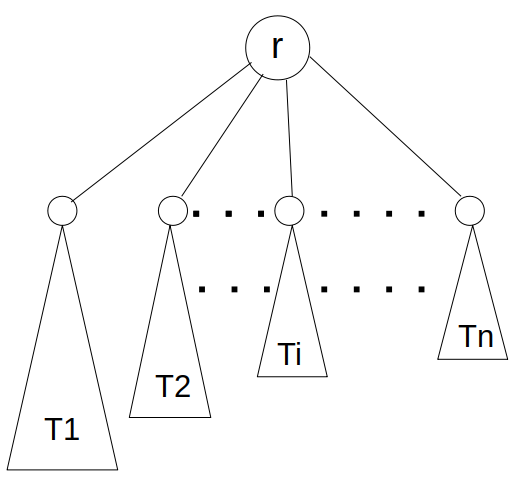
\includegraphics[width=5cm]{capitolo3/grafo3}
	\caption{Esempio di albero $ T $ radicato in $ r $, con $ k $ nodi, valido come input per l'algoritmo \ref{algoritmo1}} 
	\label{fig:3}
\end{figure}
\mbox{}\\

\begin{algorithm}[H]
	\label{algoritmo1}
	\SetAlgoLined
	\caption{Decomposizioni $ f(k) $-bilanciate }
	\textbf{input} : Albero $ T $ con $ k $ nodi ;\\ 	
	$ r $ = radice di $ T $;\\
	$ n $ = numero di figli di $ r $;\\ 
	Sia $ |T_i| $ il generico albero radicato in un figlio $ i $ di $ r $ :  $ S=\sum_{i=1}^{n}|T_i| $;\\
	\For{$ i = 1,\dots,n $}
	{
		\If{$ \sum_{j=1}^{i}{|T_j|} > \frac{2}{3}\cdot S $}
		{
			$ T'\longleftarrow $ sottoalbero di  di $ T $ indotto da $ \{r\} \cup \bigcup_{j=1}^{i-1}V(T_j)$;\\
			$ T''\longleftarrow $ sottoalbero di $ T $ indotto da $ V(T) \diagdown T'$;\\
			\textbf{return} ($ T',T'' $);\\
		}	 
}
\end{algorithm}\mbox{}\\

Una volta concluso l'algoritmo \ref{algoritmo1} si avr\`a una coppia $ (T',T'') $ tale che : $ \max (|T'|,|T''|) \le f(k) $.

In base a tutte le nozioni fino ad ora discusse si pu\`o dare il seguente risultato.\mbox{}\\



\newtheorem{teorema1}[definizione]{Teorema}
\begin{teorema1}
	\label{teorema1 cap3 sez1}
Per ogni albero T di k nodi esiste un nodo r di T  tale che l'albero $T_r$, ottenuto radicando T in r, ammette una decomposizione $ (\lfloor \frac{2}{3}(k-1) \rfloor + 1)$-bilanciata ed, inoltre, sia $ (T',T'')$ tale decomposizione risulta che $ |T'| \ge 2+\frac{(k-1)}{3} $
\end{teorema1}\mbox{}
\begin{proof}
	
	Sia $ T $ un albero di $ k $ nodi,con $ k\ge 3 $ (per $k\le2$ la propriet\`a \`e banalmente vera) \\
	La prima operazione da compiere \`e individuare il nodo $ r $ di $ T $ su cui si andr\`a poi a radicare il nuovo albero $ T_r $.\\
	Si suppone che tale nodo sia un centroide dell'albero $ T $, indicato con $ r $.\\
	Sia $ T_r$ l'albero $ T $ radicato in $ r $ \\ 
	Inoltre, si suppone che i sottoalberi radicati nei figli di r siano ordinati in maniera non crescente.\\
	Si applichi a $ T_r $ l'algoritmo \ref{algoritmo1} precedentemente descritto.\\
	Sia $ \{T_i \ | \  i=1,\dots,n\} $ l'insieme dei sottoalberi radicati negli $ n $ figli di $ r $ e si consideri il primo valore di $ i $ tale che la condizione dell'$ if $ di riga $ 6 $ nell'algoritmo \ref{algoritmo1} risulti vera (si noti che tale valore di $ i $ esiste sempre dal momento che per $ i = n $ la condizione \`e verificata).\mbox{}\\\\
	Sia 
	\[ S = \sum_{j=1}^{n}{|T_i|} = (k-1 ) \]\\
	e sia
	\[ x = \sum_{j=1}^{i-1}{|T_j|} \]\\
	Distinguiamo due casi
	\begin{itemize}
	\item $\textbf{ i>2 }$ Si ha che
	\\ 
	\begin{equation}\label{1}
		x+|T_i| > \frac{2}{3}\cdot S
	\end{equation}
\\
	Inoltre per l'ordine in cui i sottoalberi $ T_i $ sono considerati
\\	
	\begin{equation}\label{2}
	|T_i| \le \frac{S}{i} \le \frac{S}{3}	
	\end{equation}
\\		
	Sottraendo la disequazione \eqref{2} alla \eqref{1} si ottiene che 
	\\
	\begin{equation}\label{3}
	x > \frac{2}{3}\cdot S - \frac{S}{3} = \frac{S}{3}	
	\end{equation}
 	\item $ \textbf{i=2} $ Anche in questo caso come nel precedente vale la disequazione \eqref{1}.\\
 	Inoltre, essendo $ i = 2 $ per costruzione dell'albero $ T $ si pu\`o dire che
 	\\
 	\begin{equation}\label{4}
 	x = |T_1| \ge |T_2| = |T_i|
 	\end{equation}
 	\\
 	Pertanto, sfruttando la disequazione \eqref{4} combinata con la \eqref{1} si ha che
 	\\
 	\begin{equation}\label{5}
 	2x > \frac{2}{3} \cdot S \Rightarrow x > \frac{S}{3}
 	\end{equation}
	\end{itemize}
Per entrambi i casi otteniamo che 
\\
\[ x > \frac{S}{3} \]
\\
Dal momento che $ x $ \`e intero otteniamo 
\\
\[ x \ge \left\lfloor \frac{S}{3}\right\rfloor  + 1\]
\\
Pertanto si avr\`a che 
\\
\begin{equation}\label{6}
	\left\lfloor \frac{S}{3}\right\rfloor  + 1 \le x \le \left\lfloor \frac{2}{3}\cdot S \right\rfloor
\end{equation} 
\\
dove $  x \le \left\lfloor \frac{2}{3}\cdot S \right\rfloor $ \`e banalmente verificata per la scelta di $ i $.
\\
Quindi 
\\
\begin{equation}\label{7}
|T'| = 1+x \le 1 + \left\lfloor \frac{2}{3}\cdot S \right\rfloor = 1 + \left\lfloor \frac{2}{3} \cdot (k-1) \right\rfloor	
\end{equation}
\\
e
\\
\begin{equation}\label{8}
|T''| = 1 + S - x = 1+S-1 - \left\lfloor \frac{S}{3}\right\rfloor = \left\lceil \frac{2}{3}\cdot S \right\rceil = \left\lceil \frac{2}{3} \cdot (k-1) \right\rceil 	
\end{equation}
\\
Poich\`e
\\
\[1 + \left\lfloor \frac{2}{3} \cdot (k-1) \right\rfloor \ge \left\lceil \frac{2}{3} \cdot (k-1) \right\rceil \] 
\\
Possiamo concludere che
\\
\[ \max\{|T'|,|T''|\} \le 1 + \left\lfloor \frac{2}{3} \cdot (k-1) \right\rfloor \]
\\
Infine da \eqref{6} segue che
\\
\[ |T'| = 1+ x \ge 1+ (1 +  \left\lfloor \frac{S}{3}\right\rfloor ) = 2 +  \left\lfloor \frac{(k-1)}{3}\right\rfloor\]
\\ 	 
\end{proof}\mbox{}\\\\
 
 	
\section{Algoritmo}
\label{cap:3 par:2}
In questa sezione si vede come \`e stato utilizzato il risultato del paragrafo \ref{cap:3 par:1} per ottimizzare e migliorare l'algoritmo \ref{algoritmo} descritto nel capitolo \ref{cap 2} (paragrafo \ref{section1}).\\
Quello che si faceva in precedenza era, dato un albero $ T_C $, con $ T $ un albero colorato radicato di $ k $ nodi i cui colori giacciono in $ C $, si procedeva al conteggio delle occorrenze di $ T_C $ nel seguente modo
\[	c(T_c,v)=\frac{1}{\beta_T}\sum_{(u,v)\in E}\sum_{\substack{C' \subset C \\C'' = C \setminus C' \\ |C'|=|T'|, |C''| = |T''|}}c(T'_{C'},v)\cdot c(T''_{C''},u) \]\\
con $ T' $ e $ T'' $ due alberi colorati, radicati rispettivamente in $ v $ ed $ u $ tali che, l'albero $ T' $ avesse un numero di nodi pari ad $ i $, con $ i = 1, \dots , k-1 $, mentre l'albero $ T'' $ avesse un numero di nodi pari a $ k-i $.

In questa nuova versione, invece, $ T_C $ viene suddiviso in due alberi $ T' $ e $ T'' $ tali da  rispettare il principio delle decomposizioni bilanciate e pi\`u nello specifico il teorema \ref{teorema1 cap3 sez1}.\\
Innanzitutto si determina se l'albero $ T_C $ \`e radicato in uno dei centroidi, nel caso in cui ci\`o non fosse vero, l'albero $ T_c $ non viene conteggiato.\\
Successivamente viene suddiviso $ T_C $ in due alberi $ T'_{C'} $ e $ T''_{C''} $ tali che: entrambi gli alberi risultino radicati nella stessa radice $ r $ di $ T $, il $ \max\{|T'|,|T''|\} \le 1 + \left\lfloor \frac{2}{3} \cdot (k-1) \right\rfloor $ e che $ |T'| \ge 2+\left\lfloor\frac{k-1}{3} \right\rfloor $.
Inoltre i due insiemi $ C' $ e $ C'' $ dovranno essere tali che $ C' \cap C'' = \{c_r\} $, dove $ c_r $ il colore del nodo radice.\\
Come nel caso precedente, l'algoritmo che si utilizza per il conteggio delle occorrenze dei $ k $-treelet colorati in $ G $ utilizza la tecnica della programmazione dinamica, quindi si procede dai sottoproblemi pi\`u piccoli arrivando a quello pi\`u grande.\\
Anche qui per ogni nodo $ v $ si inizializza $ c(T_{C_0} , v) = 1 $, dove T \`e il treelet di 1 nodo e $ C_0 = \{c_v\} $.
Questa volta, per\`o, per calcolare le occorrenze dei $ k $-treelet radicati in ogni $ v \in V $ di $ G $ non sar\`a necessario aver valutato tutte le occorrenze dei treelet fino a $ k-1 $, ma sar\`a necessario calcolarli solo fino a $ \left\lfloor \frac{2}{3}(k-1)\right\rfloor +1 $.
Tale conteggio verr\`a eseguito sulla base dell'algoritmo \ref{algoritmo} di sezione \ref{section1}. \\
Per calcolare per ogni nodo $v \in V  $ di $ G $ il numero $ c(T_C,v) $ di occorrenze dei $ k $-treelet (non indotti) radicati in $ v $ isomorfi a $ T $ i cui colori giacciono nell'insieme $ C $, invece, si suddivide $ T $ in $ (T',T'') $ in modo che tale decomposizione risulti bilanciata come descritto in precedenza e si procede al calcolo nel modo seguente\\
\[c(T_C,v) = \frac{1}{\gamma_T}\sum_{\substack{{(T',T'') \ bilanciati}\\{C' \cap C'' = \{c_r\}}}} c(T'_{C'},v)\cdot c(T''_{C''},v) \] \\
con $\gamma_T$ la nuova costante di normalizzazione che \`e uguale a $ \binom{p}{q} $, dove $ p  $ \`e il numero di sottoalberi di $ T $ isomorfi al sottoalbero radicato nell'ultimo figlio della radice di $ T' $ e $ q $ il numero di sottoalberi radicati a partire dal primo figlio della radice di $ T'' $ isomorfi al sottoalbero radicato nell'ultimo figlio della radice di $ T' $.
Di seguito viene riportato lo pseudocodice dell'algoritmo precedentemente descritto.\\\\  
\scalebox{0.75}{
\begin{algorithm}[H]
	\label{algoritmo2}
	\SetAlgoLined
	\caption{Fase di costruzione}
	\textbf{input} : Grafo $ G =(V,E) $, dimensione del treelet $ k $;\\		
	\For{$ h = 1$ to $ \left\lfloor \frac{2}{3}(k-1) \right\rfloor +1 $}{
	Si calcolano le occorrenze secondo quanto riportato nell'Algoritmo \ref{algoritmo};\\
	}

	\For{$ v \in V $}{
	\ForEach{$ T : |T| = k $}{
		Sia $ c $ un centroide di $ T $;\\
		\If{$ c \ != \ v $} {\textbf{break}; }
		Suddivido $ T $ in due alberi $ T' $ e $ T'' $ come descritto in precedenza;\\
			\[c(T_C,v) = \frac{1}{\gamma_T}\sum_{\substack{{(T',T'') \ bilanciati}\\{C' \cap C'' = \{c_r\}}}} c(T'_{C'},v)\cdot c(T''_{C''},v)\]
	}	
} 	
\end{algorithm}
}\mbox{}\\

Come in algortimo \ref{algoritmo} le occorrenze di $ T $ sono calcolate con un approccio basato sulla scomposizione dell'albero in due sottoalberi,  per\`o, anche in questo caso nella tesi l'algoritmo \ref{algoritmo2} \'e stato sviluppato nel verso opposto, ossia a partire dai conteggi di due sottoalberi $ T' $ e $ T'' $ si \`e ottenuto i conteggi relativi a $ T $.
Perci\`o per calcolare le occorrenze dei $ k $-treelet in $ G $, $ \forall v \in V $ di $ G $ si prendono tutte le possibili coppie di alberi colorati $ (T'_{C'}, T''_{C''} )$ radicate in $ v $ tali che: $ 2+ \left\lfloor \frac{(k-1)}{3}  \right\rfloor \le |T'| \le \left\lfloor \frac{2}{3}(k-1) \right\rfloor  +1 $ e $ |T''| = k-|T'| $.
Prima di poterle unire nell'albero $ T_C $ bisogna fare le opportune verifiche, ossia:
\begin{itemize}
	\label{prova}
	\item bisogna verificare che la coppia $ (T',T'') $ sia una decomposizione bilanciata per $ T $.
	Pertanto dovr\`a risultare che $ |T'| - 1 \le \left\lfloor\frac{2}{3}(k-1)\right\rfloor $ e che aggiungendo a tale quantit\`a la cardinalit\`a del sottoalbero radicato nel primo figlio di $ T'' $, denotata con $ t'' $, si abbia che $ |T'| + t'' - 1 \ge \left\lfloor\frac{2}{3}(k-1)\right\rfloor $.
	\item Anche in questo caso bisogner\`a garantire l'ordinamento sulla struttura dell'albero.
	Pertanto non sar\`a possibile unire $ T' $ e $ T'' $ se la dimensione del sottoalbero radicato nell'ultimo figlio della radice di $ T' $ \`e minore del sottoalbero radicato nel primo figlio della radice di $ T'' $.
	\item Bisogna garantire che sia rispettato il vincolo sui colori $ C' \cap C'' = \{c_v\}$, ossia i due insiemi condividono esclusivamente in colore della radice $ v $, che \`e la stessa per entrambi. 
	\item bisogna verificare che un nodo $ v $ sia il centroide dell'albero $ T $ risultante dall'unione di $ T' $ e $ T'' $.
\end{itemize}
Queste condizioni sono necessarie affinch\`e l'unione tra gli alberi $ T'_{C'} $ e $ T''_{C''} $ produca un albero valido $ T_C $.

Come si nota, anche in questo caso, i conteggi inizialmente vengono fatti su ogni $ v\in V $, ma poich\`e in questa tesi interessano le occorrenze dei diversi $ k $-treelet su tutto $ G $  sar\'a necessario aggregare gli alberi radicati su ogni $ v $ di $ G $, unendoli a seconda della propria struttura e sommando le rispettive occorrenze.

Nel caso in cui si abbiano due centroidi, la scelta su quale radicare l'albero  \`e deterministica.\\
Nel caso in cui gli alberi ottenuti radicando $ T $ in ognuno di essi abbiano strutture differenti, viene scelto quello che tra i due ha una struttura pi\`u piccola.
Altrimenti se gli alberi ottenuti sono identici, viene scelto uno dei due in maniera arbitraria.
Questo implica che tali alberi vengano conteggiati un numero di volte doppio rispetto al conteggio reale.
Perci\`o in fase di normalizzazione i conteggi di tutti gli alberi per cui questa condizione risulta vera saranno ulteriormente divisi per due.


\section{Dettagli implementativi. Modifica e aggiunte alle rappresentazioni}
\label{cap 3:3}
Anche in questa nuova versione gli oggetti principali manipolati restano i treelet colorati e le occorrenze associate.

Ogni treelet colorato $ T_C = (T,C)$ continua ad avere una rappresentazione unica, memorizzata usando interi a 64 bit.
I bit hanno lo stesso ordinamento della precedente versione.
Quello che cambia, per\`o, \`e la suddivisione dei bit:
\begin{itemize}
	\item i bit da 0-3 contengono un valore numerico che \`e pari ad 1 se l'albero ha un solo centroide o due centroidi tali che, gli alberi ottenuti radicando $ T $ in ognuno di essi risultino diversi.
	Mentre \`e pari a  2 se l'albero ha due centroidi tali che, gli alberi ottenuti radicando $ T $ in ognuno di essi risultino uguali.
	\item  i bit da 4-7 contengono il numero $\mu$ di sottoalberi in $ T'' $ radicati a partire dal primo figlio della radice isomorfi al sottoalbero radicato nell'ultimo figlio della radice di $ T' $.
	\item i bit da 8-11 contengono il valore $ q $ necessario nel calcolo binomiale $ \binom{p}{q} $ usato in fase di normalizzazione.
	La somma di $ q $ con $\mu$ restituisce $ p $.
	\item i bit da 12-63 restano invariati alla versione precedente.	  
\end{itemize} 

La struttura dell'albero \`e codificata esattamente come la versione precedente,in particolare i sottoalberi radicati nei figli della radice dell'albero, appaiono in ordine non crescente rispetto alle relative rappresentazioni, definendo implicitamente un ordinamento totale sui treelet (colorati).\\\\
Alle precedenti operazioni sugli alberi se ne aggiungono delle nuove che sono:
\begin{itemize}
	\item $ \textbf{balance\_merge}(T',T'') $ : fa l'unione di due alberi $ T' $ e $ T'' $ in maniera bilanciata.
	All'interno del metodo viene garantito che tutte le condizioni necessarie affinch\`e l'unione avvenga, descritte in fondo al paragrafo precedente, siano verificate.
	\item $ \textbf{normalization\_factor\_balanced}(T) $ : restituisce il fattore di normalizzazione $ \gamma_T $ dell'unione bilanciata.
\end{itemize}\mbox{}\\
Un'altra differenza rispetto la versione precedente riguarda la costruzione della tabelle.
Infatti, seguendo quanto descritto in algoritmo \ref{algoritmo2}, verranno costruite tutte le entrate da 1 a  $ \left\lfloor \frac{2}{3}(k-1) \right\rfloor +1 $ come veniva fatto nella versione precedente.
Mentre non verranno costruite le $ h $ tabelle tali che: $ \left\lfloor \frac{2}{3}(k-1) \right\rfloor +1 < h < k $, ma si proceder\`a direttamente alla costruzione della tabella contenente i $ k $-treelet.\\
Anche in questa versione i treelet colorati raggiunti $ \forall v \in V $ verranno aggregati e i loro conteggi sommati ed anche in questa versione i conteggi di nodi differenti  (per ogni valore di $ h $ fissato) vengono calcolati in parallelo da pi\`u thread.